\documentclass[draft]{agujournal2019}
\usepackage{url} %this package should fix any errors with URLs in refs.
\usepackage{lineno}
\usepackage[inline]{trackchanges} %for better track changes. finalnew option will compile document with changes incorporated.
\usepackage{soul}

\linenumbers

\draftfalse

%% Enter journal name below.
%% Choose from this list of Journals:
%
% JGR: Atmospheres
% JGR: Biogeosciences
% JGR: Earth Surface
% JGR: Oceans
% JGR: Planets
% JGR: Solid Earth
% JGR: Space Physics
% Global Biogeochemical Cycles
% Geophysical Research Letters
% Paleoceanography and Paleoclimatology
% Radio Science
% Reviews of Geophysics
% Tectonics
% Space Weather
% Water Resources Research
% Geochemistry, Geophysics, Geosystems
% Journal of Advances in Modeling Earth Systems (JAMES)
% Earth's Future
% Earth and Space Science
% Geohealth
%


\journalname{JGR: Solid Earth}


\begin{document}

\title{High geomagnetic field intensity in the late Mesoproterozoic recorded by Midcontinent Rift anorthosite xenoliths}


\authors{Yiming Zhang\affil{1}, Nicholas L. Swanson-Hysell\affil{1}, Margaret S. Avery\affil{1,3}, Roger R. Fu\affil{4}}

\affiliation{1}{Department of Earth and Planetary Science, University of California, Berkeley, CA, USA}
\affiliation{2}{Department of Earth and Environmental Sciences, University of Minnesota, Duluth, MN, USA}
\affiliation{3}{Geology, Minerals, Energy, and Geophysics Science Center, U.S. Geological Survey, Moffett Field, CA, USA}
\affiliation{4}{Department of Earth and Planetary Sciences, Harvard University, Cambridge, MA, USA}
\correspondingauthor{Yiming Zhang}{yimingzhang@berkeley.edu}


\begin{keypoints}
\item New \textit{ca.} 1092 Ma Midcontinent Rift anorthosite record high paleointensity values
\item High VADM of the geomagnetic field is inconsistent with previous interpretation of Proterozoic long term decay
\item A strong geodynamo like today likely persisted for about 25 myr during the Midcontinent Rift development
\end{keypoints}


% keywords: absolute paleointensity, Laurentia, Midcontinent Rift, anorthosite, geodynamo



\begin{abstract}
New high-quality absolute paleointensity data from anorthosite xenoliths within the Beaver River diabase intrusions of the North American Midcontinent Rift (MCR) record an average virtual axial dipole moment (VADM) estimate of $\sim$80 ZAm$^2$ \textit{ca.} 1092 Ma. This cooling rate corrected paleointensity estimate from the MCR intrusive unit is similar to previous results from extrusive units that are dated to be \textit{ca.} 1108 Ma and \textit{ca.} 1085 Ma. Rock magnetic analyses and magnetic imaging reveal that the anorthosites can have abundant single-domain magnetic carriers that are ideal for paleointensity experiment, leading to a high success rate passing our selection criteria. Taken together, new and previously published paleointensity data from the Midcontinent Rift support that a geomagnetic field strength persisted through the Midcontinent Rift development and the data are inconsistent with the interpretation of a decay of Earth's geodynamo strength through the late Mesoproterozoic. 


\end{abstract}

\section*{Introduction}
%The question of the core and the importance of the observational data as complementary for numerical simulation work.

That we have a solid inner core today is the result of secular cooling and differentiation of the layered Earth. The timing of inner core formation during Earth's thermal evolution is amongst the major unsolved questions in Earth's history. Due to the uncertain constraints on the thermal conductivity of the core \cite{Konopkova2016a, Gomi2013a, Ohta2016a}, numerical simulations have given drastically different predictions on the inner core nucleation age, ranging from about half a billion years ago to prior to the Archean \cite{Pozzo2012a, Gubbins2004a, Nimmo2015a}. Some models have suggested the thermal-convection-dominated liquid core motion experienced a long-term waning before the nucleation of the inner core, which kick-started the rigorous compositional convection between the solid inner core and liquid outer core \cite<e.g>{Davies2021a}. A corollary of such a prediction is that the geomagnetic axial dipole field, which is generated by the fluid motion in the liquid core, would have experienced a long-term decay before the emergence of the solid inner core, after which a significant increase in Earth's axial dipole field strength occurred \cite{Aubert2009a, Davies2021a}. 

Paleomagnetic data from ancient rocks are one of the few types of observational data that have the potential to record the evolution of Earth’s core and can be used to test the predictions from numerical simulations. Paleointensity studies have found very low axial dipole moment (VDM) estimates from rocks formed in the late Ediacaran \cite{Bono2019a, Shcherbakova2019a, Thallner2021b}, followed by a recovery near the Ediacaran-Cambrian boundary \cite{Thallner2021a}. Other studies focusing on paleomagnetic directions have also found that the late Ediacaran might have been a period of time when the geomagnetic field were experiencing frequent reversals and waning of dipole dominance \cite{Bono2015a, Kodama2020a}. It has been interpreted that these findings are consistent with the results of geodynamo models using high core thermal conductivity values that suggest the inner core nucleation age being near the Ediacaran-Cambrian boundary \cite{Driscoll2016a, Davies2021a}. \citeA{Bono2019a} based on a polynomial fit through filtered Precambrian paleointensity database (PINT; \url{http://earth.liv.ac.uk/pint/}) to suggest the selected observational records show that the geodynamo power progressively decreased through the Proterozoic. They also recovered very low paleointensity values from \textit{ca.} 565 Ma single silicate crystals and interpreted them to be reflecting that the geodynamo reached its lowest near the Ediacaran-Cambrian boundary. Such decay trend in the Neoproterozoic is recently supported by new low paleointensity estimates derived from the \textit{ca.} 720 Ma Franklin Large Igneous Province \cite{Lloyd2021a}. 

However, previous paleointensity data from intrusive and extrusive rock units in the Mesoproterozoic Midcontinent Rift \cite{Pesonen1983a, Kulakov2013a, Sprain2018a} record Earth's virtual axial dipole moment (VADM) values similar to that of today, which are higher than the prediction of the long term decay curve (Fig. \ref{}). \citeA{Pesonen1983b} obtained an average virtual dipole moment of 93 ZAm$^2$ after applying a 13\% cooling rate correction (114 ZAm$^2$ before correction) using the \textit{ca.} 1108 Ma Osler Volcanics, Maimainse Point volcanics, intrusive Logan Sills, Thunder Bay dikes, and the Baraga and Marquette dikes, as well as the \textit{ca.} 1096 Ma North Shore Volcanic Group. \citeA{Sprain2018a} obtained more high-quality paleointensity data using the \textit{ca.} 1108 Ma Osler Volcanics and the \textit{ca.} 1100 Ma Mamainse Point volcanics. A calculated mean VADM value of 56 $\pm$ 21 ZAm$^2$ is similar to the average value of the past 300 million years. In addition, an average VADM of 59 $\pm$ 11 ZAm$^2$ obtained \citeA{Kulakov2013a} using the \textit{ca.} 1085 Ma Lake Shore Traps volcanics suggests that the present-day-like geomagnetic field strength likely persisted through the late stage of Midcontinent Rift magmatism. 

Non-ideal paleointensity behaviors at specimen level and overall low success rates have challenged the interpretation of many previous paleointensity results obtained from Midcontinent Rift rock units. One typical failure of paleointensity experiment is the double-slope behavior, as two distinct paleointensity estimates may be calculated depending on the interpreter's choice of slope: a higher paleointensity estimate from the low-temperature portion and a lower paleointensity estimate from the high-temperature portion. \citeA{Pesonen1983a} used the low-temperature slope as the best representation of the past magnetic field strength whereas \citeA{Kulakov2013a} used the high-temperature slope. Such non-ideal behavior were interpreted as failure by \siteA{Sprain2018a} who applied stricter paleointensity selection criteria and accepted only 23 out of 133 specimens (5 out of 21 lava flows) from the Osler Volcanics and the Mamainse Point volcanics. Despite the low success rate of paleointensity experiments, specimens that yield dominantly single-slope paleointensity results from the \textit{ca.} 1105 Ma Osler Volcanic Group, Mamainse Point volcanics \cite{Sprain2018a}, as well as the \textit{ca.} 1085 Ma Lake Shore Traps \cite{Kulakov2013a} suggest VADM values similar to that of the present-day \cite{Sprain2018a}. Taken together, these rock units that have been dated to span $\sim$25 myr during the development of the Midcontinent Rift magmatism \cite{Swanson-Hysell2019a} may be incompatible with the hypothesis of a ``Proterozoic dipole low" \cite{Biggin2009a}. 

Although it is typical of paleointensity experiments to suffer from low success rates, bulk plagioclase-rich rocks \cite{Selkin2000a} and single plagioclase crystals \cite{Tarduno2005a} are found to be able to produce high quality paleointensity results. It has been suggested plagioclase crystals can protect magnetic minerals that exsolved within them against thermochemical alteration during paleointensity experiments. In this study, we present new paleointensity results from ``IZZI" absolute paleointensity experiments \cite{Yu2004a} on a suite of \textit{ca.} 1092 Ma bulk anorthosite xenoliths and their diabase host rocks of the Beaver Bay Complex within the Midcontinent Rift. The anorthosite lithology yielded exceptionally high success rate thanks to the plagioclase crystals shielding the magnetic minerals within. Thermal remanent magnetization (TRM) anisotropy test, full TRM acquisition test, together with magnetic imaging show that the bulk anorthosites from the Beaver Bay Complex have low TRM anisotropy, linear TRM acquisition property, and have dominant magnetic carriers interstitial to the plagioclase and are well shielded. With more single-slope, high quality paleointensity data, we seek to compare paleointensity records from the Midcontinent Rift intrusives with those from the extrusives; to test the hypothesis that the Earth's geomagnetic dipole strength remained at high values throughout the Midcontinent Rift; and to further enrich the reliable paleointensity records during the $\sim$25 myr of Midcontinent Rift magmatic activity. 

%Retrieving paleomagnetic information from Precambrian rocks can aid in our understanding of the long-term evolution of the geodynamo. A recent paleointensity study by \cite{Sprain2018a} reported a \textit{ca.} 1.1 Ga paleomagnetic field strength similar to today based on the volcanics of the Midcontinent Rift System (MRS). That study suggested that this result is consistent with models wherein this time period of the Proterozoic is characterized by a strong rather than weak geomagnetic field. However, to further evaluating the evolution of the geomagnetic field during the Precambrian, more paleointensity data are needed. 

%The MRS emplaced a vast amount of extrusive and intrusive rocks spanning a prolonged period of $\sim$25 Myrs. \cite{Swanson-Hysell2019a} published an extensive compilation of the MRS volcanics with paired high-precision CA-ID-TIMS U-Pb geochronology and high-quality paleomagnetic directions, revealing at least two dipole reversals and rapid differential plate motion of the ancient North American plate, Laurentia, during the emplacement of MRS. The synthesized North American apparent polar wander path (APWP) was interpreted to be composed primarily of rapid plate motion \citep{Swanson-Hysell2019a}. Through comparison between paleomagnetic pole positions and the APWP, such rapid plate motion and high-precision paleomagnetic and geochronological framework revealed by the MRS volcanics can provide insights into age constraints on units with poor or no geochronology data. This framework allows for further paleomagnetic contributions beyond the Midcontinent Rift volcanics. 

\section*{Geologic Settings}
% a map of the lake superior including the pesonen units, the lake shore traps, the BRD, and the osler and mamainse, together with date compilation. 

The Mesoproterozoic North American Midcontinent Rift (MCR) is an intracontinental rift that did not result in the break-up of Laurentia. Although the protracted magmatic activity in the rift lasted form \textit{ca.} 1109 Ma to \textit{ca.} 1084 Ma \cite{Swanson-Hysell2019a}, its activity during the main magmatic stage ($\sim$1098–1090 Ma; \citeA{Vervoort2007a, Miller2013a}) was punctuated with rapid and voluminous emplacement of intrusive rocks as well as extrusive volcanics. Based on high-precision $^{206}$Pb/$^{238}$U geochronology and paleomagnetic data, \citeA{Swanson-Hysell2021a} hypothesized that the massive Duluth Complex and the coeval North Shore Volcanic group (Figure \ref{fig:Geologic_map}) formed as a result of having upwelling mantled-derived plume material encountering Laurentia's thinned lithosphere due to rifting, following an ``upside-down” drainage" which rapidly transported melt to today's North Eastern Minnesota (Figure \ref{fig:Geologic_map}; \citeA{Sleep1997a, Swanson-Hysell2014a}). The plagioclase-phyric Anorthositic Series rocks of the Duluth Complex that outcrop along an arcuate shape along Northeastern Minnesota (Figure \ref{fig:Geologic_map}) are a result of such vigorous magmatic activity. 

\begin{figure}
\centering
\noindent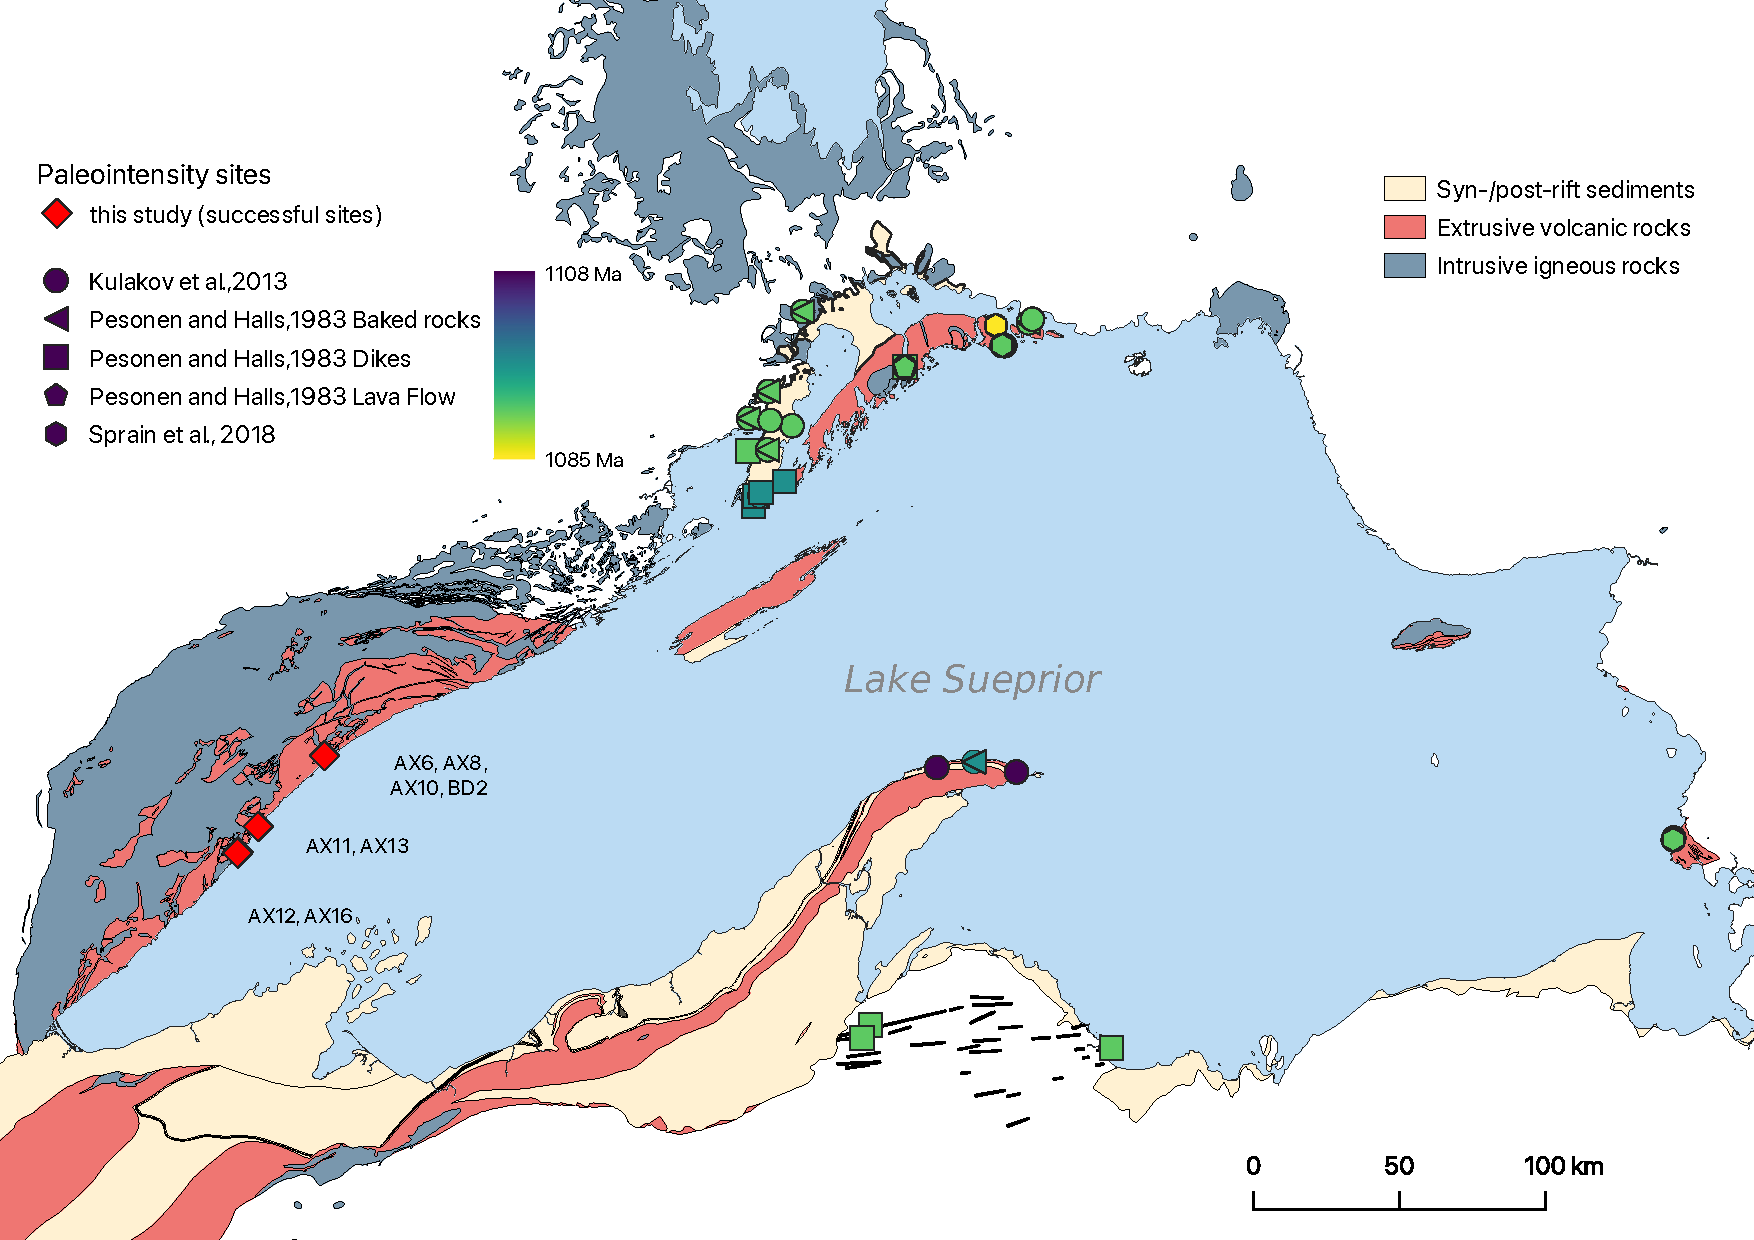
\includegraphics[width=\textwidth]{Geologic_map.pdf}
\caption{\footnotesize{Simplified geologic map of Lake Superior region showing the distribution of rift and post-rift-related rocks including extrusive, intrusive, and late/post-rift sediments around Lake Superior. Red diamonds mark sites with paleointensity results that passed the selection criteria from this study. Paleomagnetic sites from \citeA{Pesonen1983a} are categorized by lithology. All sites from previous studies are color-coded by their ages.}}
\label{fig:Geologic_map}
\end{figure}

The emplacement of the \textit{ca.} 1092 Ma Beaver Bay Complex punctuates another period of Midcontinent Rift main stage magmatism. $^{206}$Pb/$^{238}$U zircon dates and cross-cutting relationships tightly constraints the areally extensive Beaver River diabase of the Beaver Bay Complex to have been emplaced at 1091.7 $\pm$ 0.2 Ma \cite{Zhang2021b}. The Beaver River diabase intruded into hypabyssal depths via wide conduits that accommodated the entrainment of numerous anorthosite xenoliths that have short-axis diameters up to 180 meters. Geochronological, paleomagnetic, geochemical, and petrographic data are consistent with the hypothesis that the Beaver River diabase magma extruded to the surface, feeding the massive Greenstone Flow - one of the largest lava flows on Earth \cite{Doyle2016a, Zhang2021b}.

% The anorthosite xenoliths that distinctly occur within the Beaver River diabase are not only recorders of the wide diabase conduit sizes,  of the geomagnetic field $\sim$1091.7 million years ago. Thermal modeling result and paleomagnetic directional data show the anorthosite xenoliths acquired thermal remanent magnetizations during cooling of the diabase \cite{Zhang2021b}. Step-wise thermal demagnetizations show many anorthosite xenoliths have minimal secondary remanence and single-component characteristic remanence magnetizations that often unblock sharply within temperature ranges between 500\textdegree C and 580\textdegree C. 

Despite that the anorthosite xenoliths of the Beaver River diabase were entrained as xenoliths and emplaced only $\sim$4 myr after the formation of the Anorthositic Series rocks of the Duluth Complex when massive plagioclase mushes were generated, $^{206}$Pb/$^{238}$U zircon geochronology data and zircon rare earth element diffusion modeling results suggest it is the most probable that the Beaver River diabase anorthosite xenoliths are entrained cumulate enclaves that formed at the time of Beaver Bay Complex magmatism. Moreover, the anorthosite xenoliths of the \textit{ca.} 1092 Ma Beaver River diabase has distinct mineralogy from that of the Anorthositic Series rocks of the Duluth Complex. The dominantly monomineralic anorthosite xenoliths have an average anorthite content of $\sim$70\% \cite{Morrison1983a, Doyle2016a}, higher than the average of $\sim$60\% of the Anorthositic Series rocks of the Duluth Complex \cite{Miller1990a}. In addition, petrographic imaging support that the plagioclase from the Beaver River anorthosite formed under a magmatic conditions different from the Duluth Complex anorthositic series magma. While the plagioclase in the Duluth Complex Anorthositic Series typically are euhedral with an interlocking texture (Fig. \ref{Petro_QDM}), the more calcium-rich plagioclase of the Beaver River anorthosite often develop granoblastic texture characterized by equigranular plagioclase crystals (Fig, \ref{Petro_QDM}). Abundant magnetite and ilmenite needles that are typically 10 $\mu$m long can be found to have preferred orientations within Duluth Complex plagioclase. Vermicular titanomagnetite and ilmenite symplectic intergrowths also exist surrounding accessory olivine or pyroxene in the Duluth Complex Anorthositic Series rocks (Fig. \ref{Petro_QDM}). 

\begin{figure}
\noindent\includegraphics[width=\textwidth]{Petro_QDM.png}
\caption{\footnotesize{Thin section petrographic and magnetic images of anorthosites from Duluth Complex Anorthositic Series (left column) and anorthosite xenolith MS99033 from the Beaver River diabase (right column). Petrographic images (A-D) show Duluth Complex anorthosite have euhedral, elongate plagioclase crystals with interlocking texture and strong igneous foliation. The plagioclase can contain abundant Fe-Ti oxide needles (C) that have preferred orientations that are often parallel with the (010) planes of plagioclase. In contrast, plagioclase of the anorthosite xenolith MS99033 do not enclose oxide needles. Magnetic field maps acquired by the quantum diamond microscope (QDM) show that the oxide needles within Duluth plagioclase are strongly magnetic as evidenced through the overlapping magnetic dipole fields exerted above the oxides in (E). In comparison, the plagioclase of MS99033 is not magnetic. }}
\label{fig:Petro_QDM}
\end{figure}

Similar occurrences of magnetite and ilmenite inclusions within plagioclase have been described by \citeA{Haggerty1976a} in slowly cooled, mafic intrusions, and \cite{Scofield1986a} hypothesized that the inclusions acted as a means of buffering the melt with respect to oxygen, forming either crystallites along preexisting plagioclase substrate or as iron incorporated into the plagioclase that subsequently exsolved at subsolidus temperatures. Such a model requires that plagioclase, instead of other mafic minerals such as olivine, to be the first to crystallize from a magma and act as a sink for iron. The two-stage formation of the Duluth Complex Anorthositic Series fits this model \cite{Miller1990a}. During the first stage, high pressure at subcrustal depths (15-25 km depth) caused fractionation of Duluth Complex magma resulting in the formation of floating plagioclase mushes \cite{Kushiro1980a}. The second stage of crystallization then occurs at low pressures after the magma intruded into shallower chambers. 

This proposed magmatic evolution of the Duluth Complex is in distinct contrast to the emplacement of the Beaver River diabase which rapidly ascended and entrained the anorthosite xenoliths directly into shallow chambers \cite{Flower1980a, Miller1997a, Zhang2021b}. Particularly, \citeA{Miller1997a} observed a high state of structural disorder within plagioclase of the Beaver River anorthosite using X-ray diffraction analyses. This is consistent with the interpretation that these anorthosite were rapidly transported into shallow magma chambers without reaching structural equilibrium. Within the Beaver River anorthosite xenoliths, the titanomagnetite needles and the symplectic magnetite-ilmenite intergrowths are absent (Fig. \ref{Petro_QDM}). Instead, relatively sparse titano-magnetite cinterstitial to the plagioclase are typical of Beaver River anorthosites (Fig, \ref{}). 

% Previous studies have divided magmatic activity in the rift into four stages based on interpreted changes in relative magmatic volume and the nature of magmatism: early ($\sim$1109–1104 Ma), latent ($\sim$1104–1098 Ma), main ($\sim$1098–1090 Ma) and late ($\sim$1090–1084 Ma)  In particular, the main stage magmatism is characterized by rapid and punctuated events which resulted in voluminous emplacement of intrusive rocks as well as coeval outpouring of extrusive lava flows. One example is the massive \textit{ca.} 1096 Ma Duluth Complex and the North Shore Volcanic Group \cite{Swanson-Hysell2020a}, the majority of which emplaced within $<$500 kyrs. Another one is the \textit{ca.} 1092 Ma Beaver Bay Complex. The Beaver River diabase intrusions of the complex formed synchronously with the Greenstone Flow of the Portage Lake Volcanics which is one of the largest lava flows known on Earth \cite{Zhang2021b}. Excellent rock preservation thanks to minimal post-rift alteration in the Midcontinent Rift have yielded high-quality paleomagnetic directional data which have now been paired with high-precision zircon geochronology to reconstruct the ``Keweenawan Track" - a well-resolved Laurentia's (cratonic North America) apparent polar wander path during the late Mesoproterozoic \cite{Swanson-Hysell2019a}. 




\section*{Method}


\subsection*{Sample collection and paleomagnetic directions}

We collected paleomagnetic cores that are 2.5 cm in diameter along the southern and eastern Beaver Bay Complex with a particular focus on acquiring paired sites of anorthosite xenoliths and their local diabase hosts during summer field seasons in 2019 and 2020. Sample cores were collected using a hand-held gasoline-powered drill and were oriented using a magnetic compass as well as a sun compass when possible. Sun compass orientations were preferentially used for determining the sample azimuth. Specimens from a total of 7 diabase and 14 anorthosite sites were used for paleointensity experiments (Table \ref{tab:Pmag_site_data}). Sister specimens underwent step-wise alternating field (AF) or thermal demagnetization at the UC Berkeley Paleomagnetism Lab and the results are presented in \citeA{Zhang2021b}. Paleomagnetic direction measurement level data are available within the MagIC database (\url{https://earthref.org/MagIC/doi/10.1029/2021GC009909}). The close directional similarities between the anorthosite xenolith and their host diabase, the overall cooling unit mean directions between the two lithologies, and thermal modeling results are consistent with the interpretation that the Beaver River diabase and anorthosite xenoliths acquired primary thermal remanent magnetization \textit{ca.} 1092 Ma during cooling after the emplacement of the diabase \cite{Zhang2021b}. Based on the anorthosite thermal demagnetization results we selected sites whose unblocking temperature ranges are narrow and near 580\textdegree C. Beaver River diabase sites with minimal secondary remanence component were also selected for paleointensity experiments.

\subsection*{Paleointensity experiment}
A total of 69 specimens from 7 diabase sites and a total of 86 specimens from 14 anorthosite xenoliths underwent paleointensity experiments that followed the step-wise double-heating Thellier method \cite{Thellier1959a} using the IZZI protocol \cite{Tauxe2004a} with heating steps up to 585 \textdegree C. Partial thermal remanent magnetization (pTRM) checks were performed systematically throughout the experiment to test whether there was significant mineralogical alteration due to heating and were assessed using the SCAT parameter of \citeA{Shaar2013a}. On top of the IZZI modification of the Thellier experimental protocol, we also performed a comparative study where we added an extra step of 20 mT alternating field (AF) cleaning on some of the specimens after each in-field step. The purpose is to study whether the AF cleaning could help improve experiment success rate by removing the remanence component carried by materials such as multi-domain (MD) or vortex state grains that often contributes to non-ideal paleointensity behaviors. All remanence measurements were made on a 2G Enterprises DC-SQUID superconducting rock magnetometer equipped with an automated sample changer system at the UC Berkeley Paleomagnetism laboratory. The magnetometer is housed inside a three-layer magnetostatic shield that maintains background fields of less than 500 nT. Heating steps were performed using an ASC TD-48SC thermal demagnetizer with a controlled field coil that allows for a magnetic field to be generated in the oven in conjunction with a DC power supply. The thermal demagnetizer was degaussed with an alternating field in the axial orientation following each in-field step such that residual fields within the oven were $<$10 nT during zero-field steps. Samples were placed in the same location within the thermal demagnetizer for each heating step and were maintained in the same orientation with regard to the applied field. During each heating step, samples remained at peak temperatures for 20 min. An applied laboratory field of 30 μT was used for all in-field steps. All heating steps were performed in air. The temperature increments for the experiments were chosen to cover characteristic remanent magnetizations held by (titano)magnetite informed by the previous demagnetization data, with smaller increment temperature steps performed close to the expected unblocking temperature of stoichiometric magnetite \cite{Zhang2021b}. 

After the paleointensity experiment were finished, the same specimens underwent additional TRM anisotropy check with full TRMs given at 0, 30, 60, 90, 120, 150 degrees in the horizontal plane in specimen coordinates. After that, full TRM acquisition experiments were performed on the same specimens with applied fields of 30, 50, 70, and 90 $\mu$T along specimen vertical axis. 

\subsection*{Paleointensity result selection}
The following criteria were used as quality filters on the paleointensity results: (1) a maximum angular deviation (MAD; \citeA{Kirschvink1980a}) of <20\textdegree; (2) scatter parameter ($\beta$; \citeA{Coe1978a}) values of $<$15 per cent; (3) a deviation angle (DANG; \citeA{Tanaka2003a, Tauxe2004a}) of $<$5\textdegree; (4) fraction of remanence fitted for paleointensity estimate (FRAC; \citeA{Shaar2013a}) $>$0.6; (5) scatter statistic (SCAT; \citeA{Shaar2013a}) = TRUE; (6) a maximum gap (GAP-Max; \citeA{Shaar2013a}) < 0.6; (7) number of pTRM checks > 2; (8) and number of measurements used for paleointensity determination $≥$ 4. The criteria are also summarized in Table \ref{tab:criteria}. The MAD measures the scatter about the best-fit line through NRM steps in the selected interval for which the intensity is defined. DANG, the deviation angle, is the angle between the best-fit direction that is free floating and the direction between the centre of mass of the data and the origin of the vector component diagram (\citeA{Tanaka2003a}; \citeA{Tauxe2004a}). Both MAD and DANG assess the directional variation of the NRM, with MAD measuring the scatter in the NRM directions and DANG assessing whether the component is trending toward the origin of the Zijderveld plot. $\beta$ is the ``scatter" parameter of \citeA{Coe1978a} and is the ratio of the standard error of the slope of the best-fit line of the selected NRM and pTRM points on an Arai plot to the absolute value of the slope. FRAC is the fraction of the NRM that is used in the best-fit line \cite{Shaar2013a}. The FRAC value was chosen to preferentially select samples with dominantly single-slope Arai plots. GAP-Max is the maximum gap between two points on the Arai plot determined by vector arithmetic. SCAT is a Boolean operator which uses the error on the best-fit slope of the selected data on the Arai plot to determine if the data are overly scattered. The parameter is used to assess pTRM checks in addition to assessing the degree to which IZZI steps are zigzagged. $\beta$, FRAC, GAP-Max and SCAT are all statistics to assess the behavior of Arai plots. See the Standard Paleointensity Definitions (\citeA{Paterson2014a}, \url{https://earthref.org/PmagPy/SPD/home.html}) for more details. Data analysis was conducted using Thellier GUI \cite{Shaar2013a} within the PmagPy software package \cite{Tauxe2016a}.

\begin{table}
\caption{Quality criteria used for accepting or rejecting paleointensity data. See the text for more detail.} 
\centering
\begin{tabular}{ccccccccc}
\hline
MAD (o) & Beta (per cent) & DANG (o) & FRAC& SCAT & GAP-MAX & NpTRM & N Arai\\
\hline
20 & 15 & 5 & 0.6 & TRUE & 0.6 & 2 & 4 \\
\hline

\end{tabular}
\label{tab:criteria}
\end{table}



\subsection*{Rock magnetic experiment}

In this study, we conduct rock magnetic experiments with a purpose of gaining magnetic mineralogy insight into the paleointensity results of the anorthosite and diabase. Backfield curves were measured at room temperature using a Micromag Princeton Measurements vibrating sample magnetometer (VSM) with nominal sensitivity of $5 \times 10^{-9}$ Am\textsuperscript{2}, and a Lake Shore 8600 series VSM with nominal sensitivity of xxxxxxxxxx. The calculated coercivity spectra were subsequently decomposed into one ore more components using skew-normal distributions following the method of \citeA{Maxbauer2016a}. The fitted components are then used to interpret the characteristics of different populations of magnetic particles within specimens. We also used the magnetic property measurement system (MPMS) at the IRM to aid in the identification of magnetic mineral. In the field-cooled (FC) experiments shown in Figure \ref{fig:MPMS}, the magnetization was measured upon warming following the specimen having cooled in an applied field of 2.5 T from 300 to 10 K. In the zero-field-cooled (ZFC) experiment, a low-temperature saturation isothermal remanence (LTSIRM) of 2.5 T was applied at 10 K after the specimen cooled in a (near-)zero field. In the room-temperature saturation isothermal remanence (RTSIRM) experiment, the sample was pulsed with a 2.5 T field at room temperature ($\sim$300 K) and then cooled to 10 K and warmed back to room temperature in a (near)zero field. The magnetic moment transitions at critical temperatures revealed through MPMS experiments are used to identify magnetic minerals such as magnetite \cite{Verwey1939a} within specimens. 
% it would actually be nice to show the MPMS data (although it could be a bit redundant). The MPMS data nicely shows the BD and failed AX have the Verwey transition suppressed to lower temperatures and the successful AX have Verwey transition close to 120 K - the typical value for stochiometric magnetite. I don't think I will be using the hysteresis loops.


\section*{Results and Discussion}
\subsection*{Paleointensity}

40 from a total of 86 anorthosite specimens and 9 out of a total of 69 diabase specimens passed our paleointensity selection criteria, yielding 7 anorthosite sites and 1 diabase sites with site-level paleointensity results that pass paleointensity selections. Example Arai plots are shown in Figure \ref{fig:IZZI_examples}. Summary specimen absolute paleointensity estimate and site-level weighted mean paleointensity values are shown in Figure \ref{fig:PINT_cooling_corrected}. All measurement-level paleointensity experiment data can be accessed through the MagIC database (\url{}; UPDATE WHEN DOI IS GENERATED). 

\begin{figure}[h!]
\noindent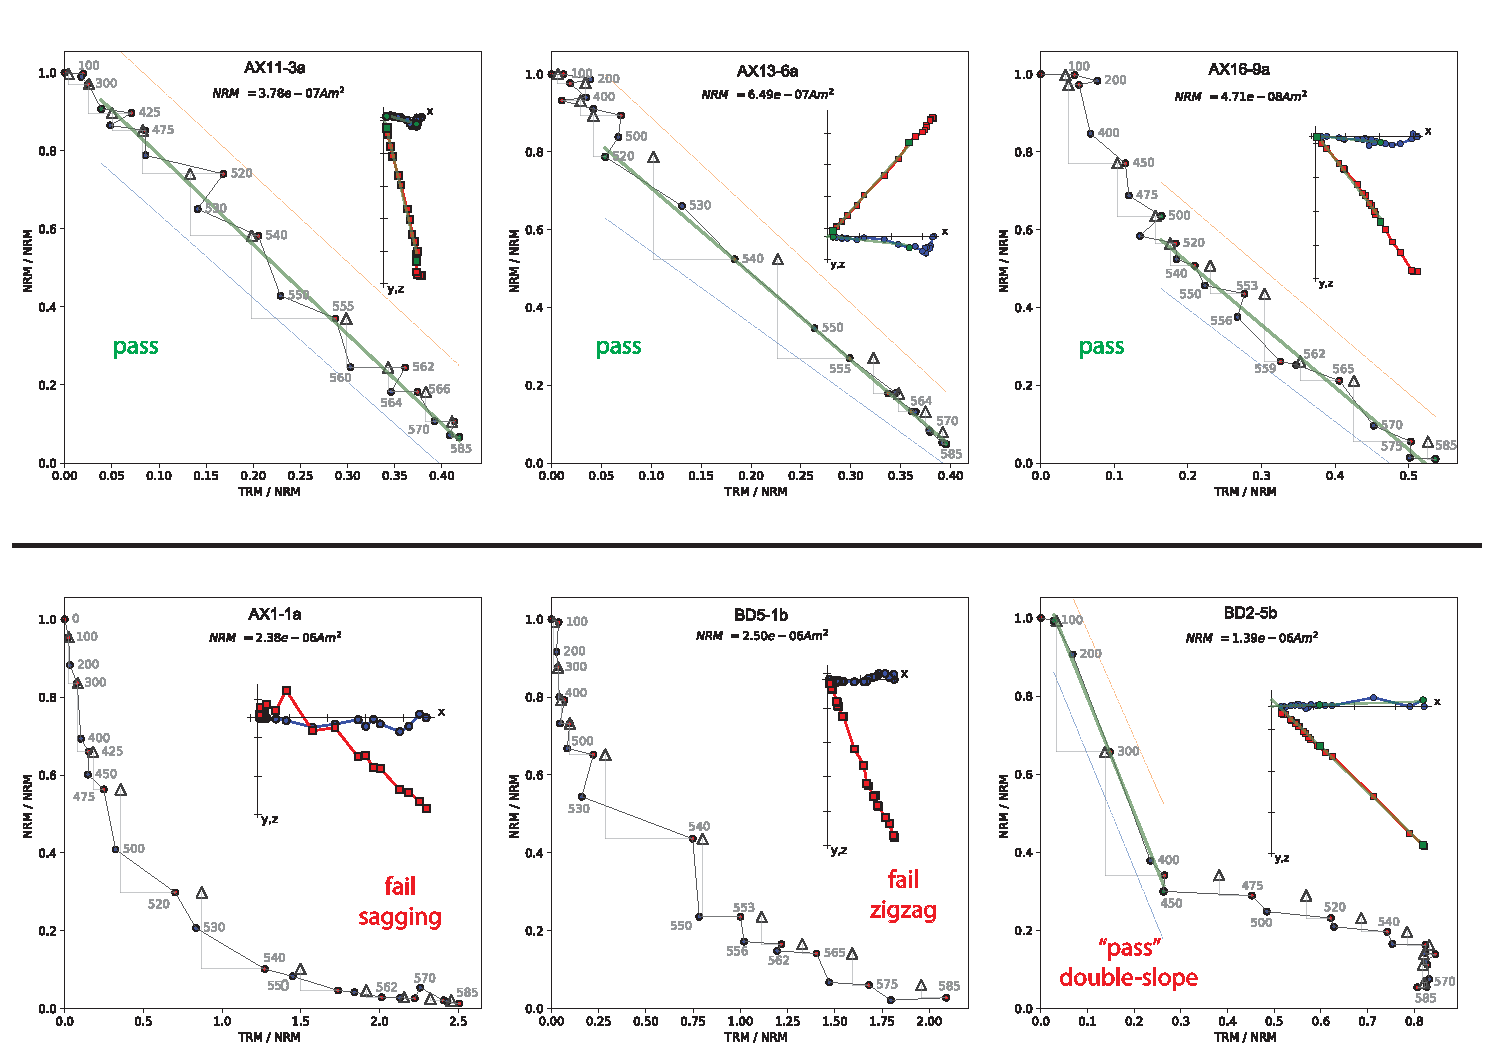
\includegraphics[width=\textwidth]{IZZI_examples.pdf}
\centering
\caption{\footnotesize{Example results of paleointensity experiments displayed on Arai and Zijderveld plots (insets) for anorthosite and diabase specimens. Red (blue) circles indicate zero-field/in-field (in-field/zero-field) steps `ZI’ (`IZ’). Triangles mark partial thermal remanent (pTRM) checks. Blue and red squares in the Zijderveld plots are X–Y and X–Z projections, respectively, of the NRMs in specimen coordinates. Plots on the top row show successful specimen paleointensity results with straight, single-slope behaviors that pass our selection criteria. The green lines represent our fitting for the dominant single-slope component that passes our acceptance criteria with estimates of the ancient field (B$_anc$) being used to determine site means. The plots for anorthosite specimens AX1-1a and diabase BD5-1b on the bottom row show typical non-ideal sagging and zigzagging behaviour that fails our acceptance criteria. Plot for diabase specimen BD2-5a shows typical paleointensity behavior of this site - specimens typically have double-slope behaviors although the lower temperature slopes can pass the selection criteria, resulting in the high estimated B$_anc$ values shown in Figure \ref{fig:PINT_cooling_corrected}. Thus, the estimates of B$_anc$ for this specimen plot is illustrative, but were not used to calculate a site mean paleointensity value in Figure \ref{fig:PINT_cooling_corrected}.}}
\label{fig:IZZI_examples}
\end{figure}

The Beaver River anorthosite specimens yielded a high pass rate ($\sim$46.5\%) through our selection criteria. In distinct contrast, the Beaver Rider diabase specimens were almost all rejected by our selection criteria. Only site BD2 has 9 specimens that passed selection ($\sim$13.0\% pass rate). Paleointensity experiment results from both lithologies show three types of dominant specimen behaviors on Arai plots (Figure \ref{fig:IZZI_examples}; \citeA{Arai1963a}): dominantly single-slope, double-slope, and zigzagging or sagging (Figure \ref{fig:IZZI_examples}). It is worth mentioning that almost all specimens have minimal secondary remanence component in thermal demagnetization results as shown in orthogonal plots of all zero-field steps (Figure \ref{fig:IZZI_examples}). Typical specimen paleointensity behavior of the anorthosites display straight, single-slope Arai plots and the accepted fractions of temperature steps span over the origin-trending, primary remanence components (Figure \ref{fig:IZZI_examples}). We accept all specimen- and site-level absolute paleointensity estimates from the anorthosite xenoliths. In terms of the diabase specimens, all but nine of them failed the selection because of double-slope behavior (fail FRAC selection), poor pTRM checks, and zigzagging (fail SCAT, DANG selection) Arai plots (Figure \ref{fig:IZZI_examples}). Even specimens in site BD2, the only site that passed selection, do not always display ideal Arai plots. As is shown in Figure \ref{fig:IZZI_examples}, specimen BD2-5b has a high-temperature second slope with zigzagging behavior, poor pTRM checks, and low NRM/TRM ratio, in addition to the straight slope with steep NRM/TRM ratio over the lower temperature range. Other accepted specimen results from site BD2 are from similar low-temperature fractions of Arai plots (below 500 $^\circ$C), which are different than those used in anorthosite sites (typically above 500 $^\circ$). Although the BD2 specimens' lower temperature fraction of the Arai plots are straight, the pTRM checks are consistent, and the specimen paleointensity results show within-site consistency and yield a weighted mean paleointensity estimate indistinguishable with that of anorthosite AX11 and AX13 (Figure \ref{fig:IZZI_examples}, \ref{fig:PINT_cooling_corrected}), specimens from BD2 give consistently higher paleointensity estimates than those from site AX6, AX8, and AX10, which are anorthosite xenoliths included within BD2 (Figure \ref{fig:Geologic_map}; \citeA{Zhang2021a}). This higher estimate from the diabase lithology could be attributed to the systematic bias of using the lower temperature slope of the Arai plots demonstrated in Figure \ref{fig:IZZI_examples}. 

Alternating field treatment after in-field heating steps likely improved the paleointensity behavior of diabase specimens such that they pass the selection criteria but the treatment did not result in significant success rate improvement or changes in paleointensity estimates for the anorthosites (Figure \ref{fig:PINT_cooling_corrected}). 8 out of 13 specimens from site BD2 that were subjected to AF treatment have straight low temperature slopes that pass the selection criteria, whereas only 1 from 4 specimens that were not subjected to AF treatment passes. On the other hand, 27 out of 58 ($\sim$46.6\%) anorthosite specimens that had AF treatment passed selection and 13 out of 28 ($\sim$46.4\%) specimens without AF treatment passed selection. Paleointensity estimates from specimens with or without AF treatment in anorthosite AX12, AX13, AX16 do not show significant difference (Figure \ref{fig:PINT_cooling_corrected}). Specimen plots for AX11 particularly illustrates a case where all specimens within the site yield almost the same paleointensity estimate, regardless of the AF treatment. Such consistent behavior makes the results from this site of very high confidence. 

The different effects that alternating field treatment had upon anorthosite and diabase may reflect the magnetic mineralogy difference between lithologies. Diabase likely has significant populations of MD or vortex state grains which can have relatively low coercivities and result in non-ideal paleointensity behaviors, but whose remanence contribution could be significant to the whole rock natural remanent magnetization. Upon the application of the 20 mT peak AF treatment after each in-field heating step, the remanence acquired by these grains is likely significantly removed, therefore making a straight slope of NRM/TRM during temperatures below 500\textdegree C (Figure \ref{fig:backfield}). On the other hand, the anorthosite specimens with and without AF treatment have very similar paleointensity behaviors and consistent specimen level estimates. Together with the narrow range of unblocking temperatures of their sister specimens \cite{Zhang2021b}, these data are consistent with the interpretation that the anorthosites with successful paleointensity results have a magnetic mineral assemblage that likely contain dominantly single domain, low Ti magnetite and they do not contain a significant population of MD or vortext state grains. Some anorthosite specimens and many diabase specimens still failed in result selections even though AF treatment was applied. It could be that they have a very high dominance of MD or vortex state grains with relatively moderate coercivity such that an alternating field with 20 mT peak field did not significantly mitigate their non-ideal paleointensity behaviors. Another cause for their failure could be of thermochemical alterations that happened during heating in air. As can be exampled by the zigzagging high temperature slope with poor pTRM checks in paleointensity plot for specimen BD2-5b (Figure \ref{fig:IZZI_examples}), the decrease in NRM/TRM ratios during higher temperature steps likely resulted from the formation of new ferromagnetic material within the specimen due to oxidation. Such alteration can allow specimens to acquire additional remanence during in-field steps that may not be fully removed by an AF treatment.

\begin{table}[]
\caption{\footnotesize{Summary statistics for the Q$_{PI}$ quality criteria of \citeA{Biggin2014a}.}}
\centering
\begin{tabular}{ccccccccccccc}
\hline
Site & N  & Age (Ma) & Method & AGE & STAT & TRM & ALT & MD & ACN & TECH & LITH & QPI \\ \hline
AX6  & 3  & 1091.8   & T+     & 1   & 0    & 1   & 1   & 1  & 1   & 0    & 0    & 5   \\
AX8  & 3  & 1091.8   & T+     & 1   & 0    & 1   & 1   & 1  & 1   & 0    & 0    & 5   \\
AX10 & 3  & 1091.8   & T+     & 1   & 0    & 1   & 1   & 1  & 1   & 0    & 0    & 5   \\
AX12 & 6  & 1091.8   & T+     & 1   & 1    & 1   & 1   & 1  & 1   & 0    & 0    & 6   \\
AX16 & 11 & 1091.8   & T+     & 1   & 1    & 1   & 1   & 1  & 1   & 0    & 0    & 6   \\
AX11 & 7  & 1091.8   & T+     & 1   & 1    & 1   & 1   & 1  & 1   & 0    & 0    & 6   \\
AX13 & 7  & 1091.8   & T+     & 1   & 1    & 1   & 1   & 1  & 1   & 0    & 0    & 6   \\ \hline
BD2  & 9  & 1091.7   & T+     & 1   & 1    & 1   & 1   & 1  & 1   & 0    & 0    & 6   \\ \hline
\end{tabular}
\label{tab:QPI}
\end{table}

\subsection*{Rock magnetism}
Rock magnetic data support the interpretation that the successful anorthosite specimens have dominant magnetic carriers with magnetic properties similar to stochiometric, non-interactive, single domain magnetite, whereas those anorthosites that failed the paleointensity result selection and all diabase have more pronounced non-ideal carriers. MPMS data show sister specimens to paleointensity specimens typically have dominant magnetic mineralogy of magnetite as can be evidenced through the Verwey transitions (Figure \ref{fig:MPMS}; \citeA{Verwey1939a}). However, specimens from sites that yield successful paleointensity results display Verwey transition near 120 Kelvin (K) as expected for stochiometric low-Ti magnetite (\cite{Ozdemir1993a}). On the other hand, the diabase specimens and anorthosite specimens that did not yielded accepted paleointensity results typically have suppressed Verwey transition toward lower temperatures (Figure \ref{fig:MPMS}), indicating that the specimens likely have a ferromagnetic mineralogy with relatively high Ti content and/or with variable degrees of oxidation \cite{Ozdemir1993a}. 
 
\begin{figure}[h!]
\noindent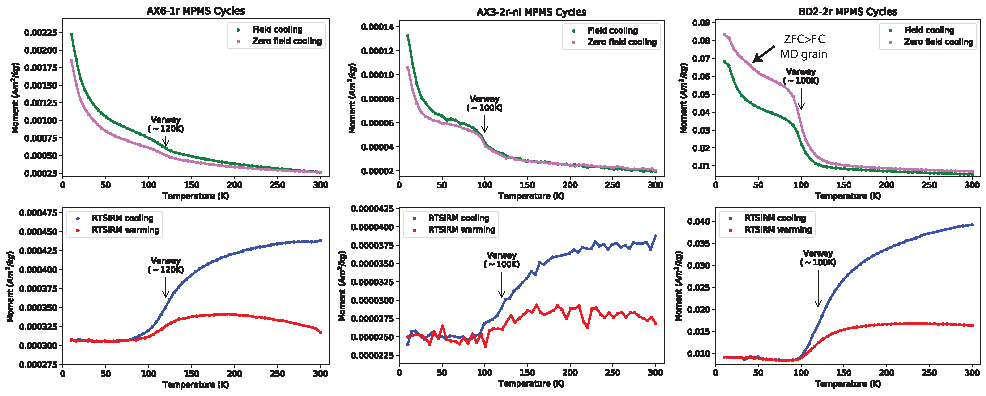
\includegraphics[width=\textwidth]{MPMS.pdf}
\centering
\caption{\footnotesize{Low-temperature magnetic property measurement system (MPMS) experiment results. In the field-cooled (FC) experiments, the magnetization was measured upon warming following the specimen having cooled in an applied field of 2.5 T from 300 to 10 K. In the zero-field-cooled (ZFC) experiment, a low-temperature saturation isothermal remanence (LTSIRM) of 2.5 T was applied at 10 K after the specimen cooled in a (near-)zero field. In the room-temperature saturation isothermal remanence (RTSIRM) experiment, the sample was pulsed with a 2.5 T field at room temperature ($\sim$300 K) and then cooled to 10 K and warmed back to room temperature in a (near)zero field. Specimen AX6-1r is from anorthosite AX6 which passed our paleointensity selection. It has a well-defined Verwey transition $\sim$120 K. Specimens AX3-2r-ni and BD2-2r have prominent Verwey transition but the transition temperatures are suppressed below $\sim$120 K. }}
\label{fig:MPMS}
\end{figure}

Specimen coercivity spectra further support that our paleointensity selection criteria are successful in selecting experiment results. A compilation of median destructive field (MDF) in Figure \ref{fig:coercivity} based on all of our backfield experiments shows that successful anorthosites have distinctly higher average MDF range than others. Example single component skew-normal distribution fits of coercivity spectra based on backfield experiments on specimen chips sister to paleointensity specimens show that anorthosites that yielded successful paleointensity results can have magnetic grain populations with peak coercivity distributions around 80 mT, very similar to that of a bulk sample composed of no-interactive single domain magnetite (Figure \ref{fig:coercivity}). In contrast, specimens from anorthosite that did not pass paleointensity selection, as well as diabase specimens, tend to have coercivity distributions over a significantly lower range ($\sim$30 mT). This is consistent with the interpretation that they lack a dominance of single domain magnetite grains in their ferromagnetic mineral assemblages.

\begin{figure}[h!]
\noindent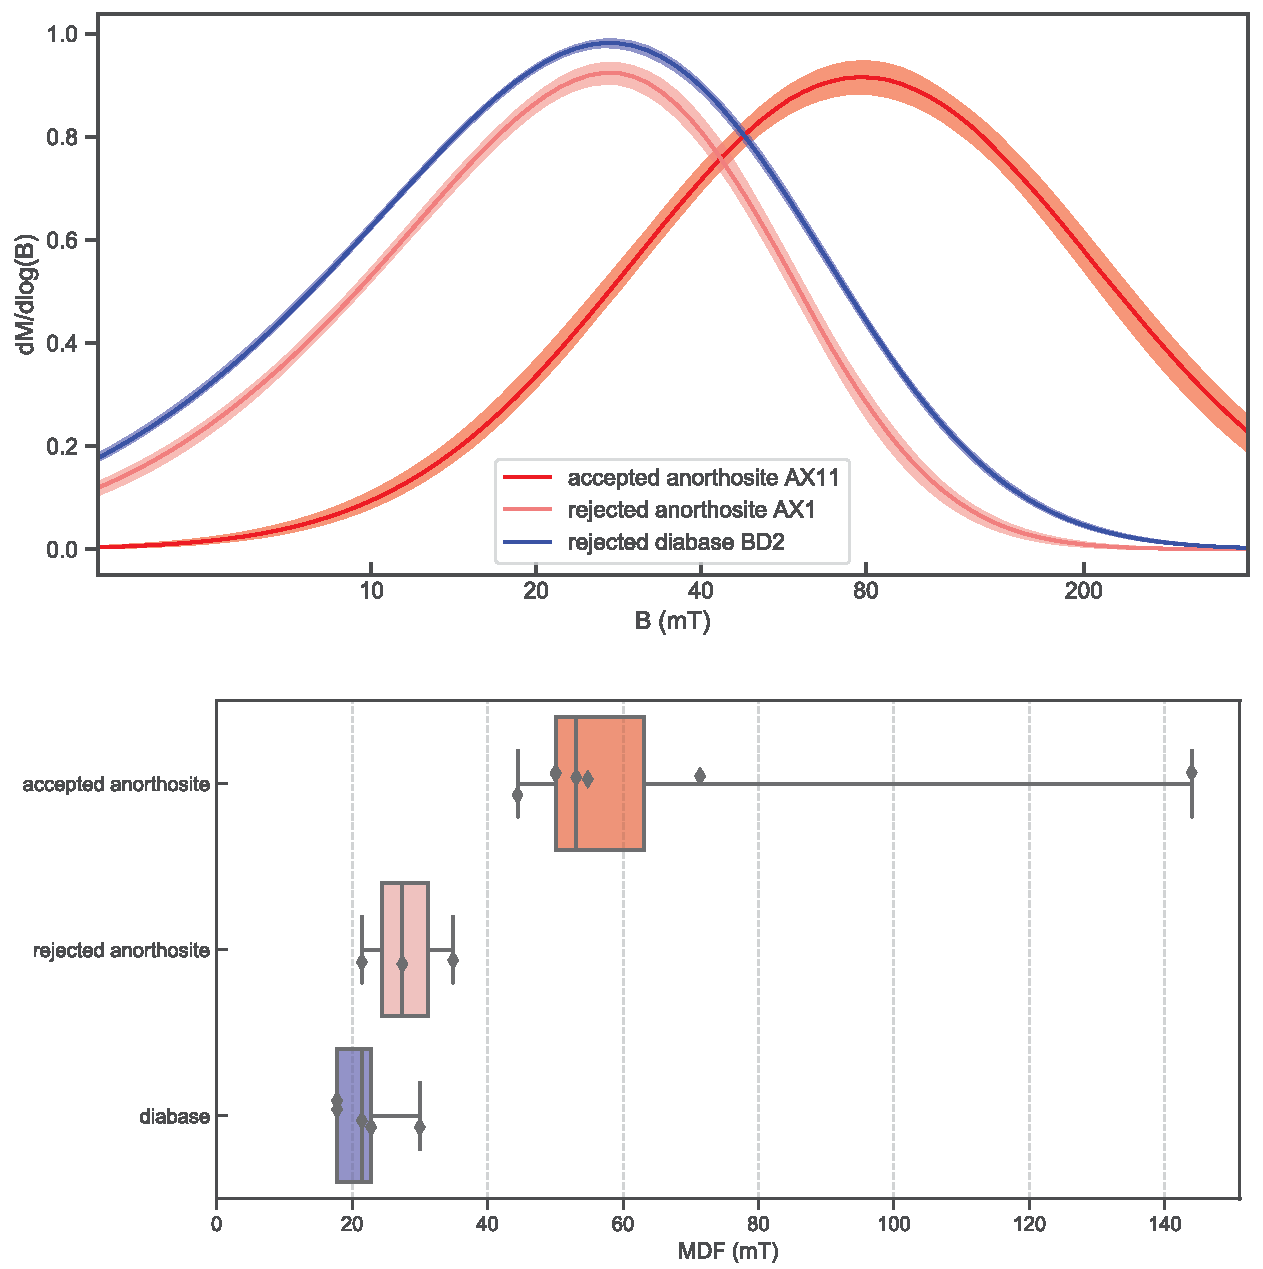
\includegraphics[width=\textwidth]{coercivity.pdf}
\centering
\caption{\footnotesize{Top: Example coercivity unmixing plots on anorthosites and diabase specimens from sites that pass or fail our paleointensity selection criteria. Bottom: Box plots summarize distributions of median destructive field (MDF) values for all anorthosite and diabase specimens that have single-component coercivity unmixing results. Both plots show that anorthosite specimens that pass our paleointensity selection criteria have distinctly higher MDF than other anorthosites that do not pass the selection, as well as all diabase specimens. The diabase site BD2 which is the only site that yielded specimen results that pass the selection, have similar MDF than other diabase sites.}}
\label{fig:coercivity}
\end{figure}

\subsection*{Remanence anisotropy and nonlinear TRM acquisition check}
Significant remanence anisotropy has been documented to exist within anorthositic rocks that form in layered intrusive rocks \cite{Selkin2000a, Feinberg2006a}. \cite{Selkin2000a} demonstrated that strong remanence anisotropy associated with the igneous foliation developed within an anorthosite sample from the Stillwater Complex can lead to paleointensity estimates that are different by three times. Depending on the orientation of the applied field during in-field steps and that of the magnetic anisotropy axes of a specimen, such strong preferred orientations of petrofabrics can result in significantly biased paleointensity estimates. To assess whether our paleointensity estimates are biased by remanence anisotropy, we first calculated the gamma statistic, which is the angular difference between the last pTRM step used for paleointensity determination and the applied field direction. The results show all anorthosite specimens used for paleointensity experiment have gamma values ranging from $\sim$0.9\textdegree-$\sim$11.9\textdegree, with a median value of 4.2\textdegree (Table \ref{}). These gamma values are similar to those of the Midcontinent Rift volcanics \cite{Sprain2018a} and they show that the Beaver River anorthosite bulk rocks do not have a significant directional remanence anisotropy. This result can be further supported by the fact that the recovered paleodirectional data from our anorthosite xenoliths closely match those from the paired Beaver River diabase hosts \cite{Zhang2021b}, the lithology of which is usually considered isotropic in terms of recording remanence magnetization. Further, we applied full TRMs to the anorthosite specimens that pass the paleointensity selection criteria after paleointensity experiment. With an applied field of 30 $\mu$T oriented toward the specimen at 0, 30, 60, 90, 120, and 150 degrees, the anorthosite specimens usually acquired consistent full TRMs. The most significant variations observed in acquired full TRMs reach to only XXX \%, much less than that has been reported to occurred within layerd anorthositic rocks in Stillwater (up to $\sim$60 \%, \citeA{Selkin2000a}). 

\cite{Selkin2007a} also noted that vortex state magnetic grains and certain single domain particles can produce biased paleointensity estimates due to their nonlinearity behavior of thermal remanence acquisition. We applied full TRMs to our anorthosite specimens with lab fields of 30, 50, 70, and 90 $\mu$T along specimen vertical axis. The results show that our anorthosite specimens did not saturate upon an applied field of 30 $\mu$T and there is thus no need for correcting nonlinear thermal remanence acquisitions.  

The reason that the Beaver River anorthosite xenoliths do not display strong remanence anisotropy, nor do they display nonlinear TRM acquisition problem, could be that they formed in a magmatic setting distinct from that of a layered mafic complex, such as the nearby Duluth Complex, where igneous foliation can occur (Figure \ref{fig:Geologic_map}). Petrographic images show that an equigranular texture where equidimensional, randomly oriented plagioclase often develop in the anorthosite xenoliths (Figure \ref{fig:Petro_QDM}; \citeA{Zhang2021b}). This is in contrast with the interlocking igneous foliation texture within the Anorthositic Series rocks of the \textit{ca.} 1096 Ma Duluth Complex (Figure \ref{fig:Petro_QDM}). Further, magnetic imaging also shows the Beaver River anorthosite xenoliths do not develop abundant magnetite and ilmenite needle exsolution within plagioclase crystals as the slowly-cooled anorthositic intrusions, in which exsolved magnetite needles can be the dominate remanence carriers (Figure \ref{fig:Petro_QDM}; \citeA{Scofield1986a, Feinberg2006a}). In addition, the aligned magnetic maps and the petrographic images in Figure \ref{fig:Petro_QDM} nicely illustrates that the magnetic dipole fields are exerted by the magnetite needles. The fact that all dipole features within a same plagioclase crystal have indistinguishable orientations is consistent with the interpretation of there being a magnetic remanence anisotropy resulting from preferred petrofabric alignment, giving rise to the remanence anisotropy and nonlinear TRM acquisition of layered anorthositic intrusions (Figure \ref{fig:Petro_QDM}). 

\subsection*{Cooling rate correction}
Paleointensity estimates from igneous intrusions can also be biased toward higher values due to slow cooling rates \cite{Halgedahl1980a}. Because the cooling rates of intrusive rocks could be much longer than the extrusive rocks, the slowly cooled diabase and anorthosite can bias laboratory paleointensity estimates toward an overestimate for SD grains \cite{Dodson1980a, Halgedahl1980a, Selkin2000a}. 

From the thermal history model we can also estimate the duration which the diabase and anorthosite cooled from the Curie temperature of magnetite ($\sim$580\textdegree C) to the time when they fully block in their characteristic natural remanence component ($\sim$500\textdegree C; \citeA{Zhang2021b}). We find the cooling time to be on the order of $\sim$1 kyr, which corresponds to a cooling rate of $1.6\times10^{-9}$ $^\circ$C s$^{-1}$. In contrast, the lab cooling rate is much faster, at about $1.3\times10^{-1}$ $^\circ$C s$^{-1}$ if we assume it takes 10 minutes in lab condition to cool through the same temperature interval. As a result, this significant cooling rate difference leads to a prediction of 35.5\% overestimate of true ancient field \cite{Halgedahl1980a}. We therefore correct our paleointensity results by a factor of 0.74. The cooling rate corrected specimen paleointensity estimates together with specimen- and site-level weighted means are shown in Figure \ref{fig:PINT_cooling_corrected}. Taking all accepted anorthosite paleointensity results, they have a site mean absolute paleointensity estimates of 47.90 $\pm$ 9.32 $\mu$T (Figure \ref{fig:PINT_cooling_corrected}). 

\subsection*{Late Mesoproterozoic geomagnetic field and the Precambrian observation records}
Figure \ref{fig:PINT_plot} shows all accepted anorthosite and diabase specimen paleointensity results and their site-level means with one standard deviation envelopes. An anorthosite site mean paleointensity weighted by site standard deviations is plotted as a dashed orange line, and the standard deviation envelope as dashed green lines. The anorthosites are also grouped by their geographical vicinity \ref{fig:PINT_plot}. The site-level results are shown in Table \ref{tab:PINT_result}. Anorthosite sites AX10, 11, 12, 13, 16 yielded very high within-site coherence (Figure \ref{fig:Arai_plots, fig:PINT_plot}), which suggest high-confidence site-level paleointensity estimates. Clearly there are two populations of paleointensity results: a group of high estimates from anorthosite site 11 and 13 which have very high within-site consistency and are in agreement with the results from BRD site 2; and another group of low estimates from anorthosite site 6, 8, 10, 12, and 16, which also have tight agreement across sites.

All units have Q$_{PI}$ scores \cite{Biggin2014a} ranging between 5 and 6 (Table \ref{tab:QPI}). All sites passed AGE, TRM and ALT (pTRM checks passed and high-temperature steps that looked to be suffering from alteration were excluded), ACN and MD (no significant sagging or zigzagging).

% need to export the figure with tight boundaries
\begin{figure}[h!]
\noindent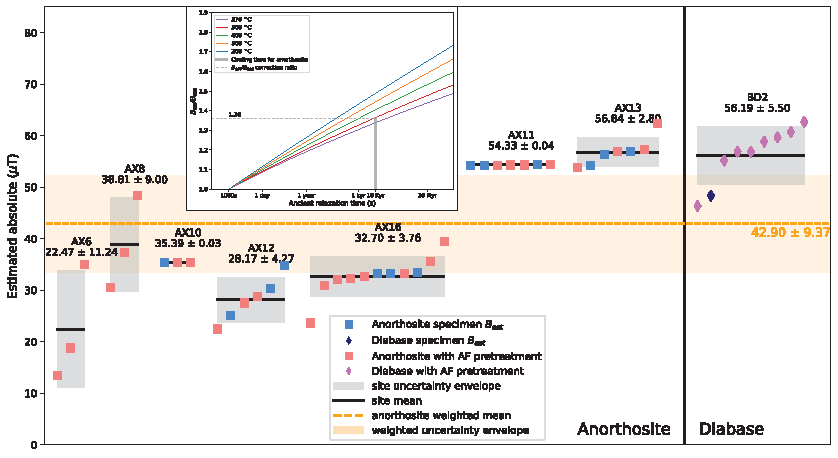
\includegraphics[width=\textwidth]{Paleointensity_plot_cooling_corrected.pdf}
\centering
\caption{\small{Summary plot of cooling rate corrected specimen absolute paleointensity results (square and diamond symbols) from this study and their weighted averages at site (grey bar) and locality level (orange bar). }}
\label{fig:PINT_cooling_corrected}
\end{figure}


considering \citeA{Nagy2021a} developed a new cooling rate correction model for uniaxial single domain magnetite and suggest that the model of \citeA{Halgedahl1980a} tend to over-correct for cooling rates and lead to underestimating ancient fields. If our absolute paleointensity values are an underestimating, 


In addition, \cite{Cych2021a} developed a Bayesian probability method to estimate paleointensity - independent of the selection criteria, the Bayesian method fits for the curvature and generate probability distribution that guides credible interval for the paleoitnensity at a site level. The result distribution of Markov Chain Monte Carlo resampling are shown as violin plots in Figure \ref{}. The cooling rate corrected distributions show similar results as the frequentists' estimates based on the selection criteria derived results. 

Address the spacial groups and using direction and intensity to address the issue of secular variation. 

overall the PINT results are of high quality and the Qpi index average to be 6 to 7. 

The calculated paleomagnetic VADM values are shown in Figure \ref{} in context of the compilation of all Midcontinent Rift results. highlight the high quality of the results and the consistency of MCR rocks' high geomagnetic field values even considering the uncertainties of previous data. Supporting that the Mesoproterozoic likely experienced a period of persistent high geomagnetic strength in addition to the protracted magmatism of in the formation of the massive intracontinental rifting. 

% cooling rate correction problem - that the Nagy et al paper can suggest even less of a correction and higher of the estimated field. theoretical thermal modeling by \citeA{Zhang2021a} suggest tha the anorthosite xenoliths were likely heated to diabase magma temperature regardless of their sizes, and cooled through the typical characteristic unblocking temperature range from 580 to 500 on the order of 1000 years. Comparing to the typical lab cooling time of about 100 seconds duirng paleointensity experiments, the significantly slower cooling rate when the NRM was acquired as the anorthosite xenoliths cooled with the diabase led to overestimate of paleointensity by up to 40\%. Overall range of correction factor can be 1.1-1.4, in any case consistent with a high field strength


% that this dataset also could have suffered from problem of averaging out secular variations, given that the mean pmag directions deviate from what is expected from the sythesized APWP, nevertheless the variations in estimate absolute paleointensity lead us to interpret that albeit close, the they intensity data were acquired at distinctly different times that are sufficiently far apart such that the surface geomagnetic field had already changed. 

% that \citeA{bono2019a} proposed an interesting trend but has problems in the directions, likely to be a short term feature of a low field during a reversal, instead of a low field as a result of long term cooling. 

% that Lloyd 2021 also presented low field that fits the trend, but they similarly have the issue of reversal, and that they do not have good control on secular variations

% Together with previously published data, the Midcontinent Rift rocks are recording 1.1 Ga earth geomagnetic field that is stronger than the mean of the past 300 Ma (Fig. \ref{}). 




\section*{Conclusion}
high success rate comparing to volcanics (more than half success sites), producing good consistent site level results, and across sites report present-day like field like today.

AF pre-treatment is helpful in that it increase the specimens/sites passing the selecting criteria, suggesting that the method likely helped improve the MD ferromagnetic carriers. 

Rock mag and petrographic data might suggest differences in terms of the value of peak field on coercivity spectra between those passed and those didn't.  

IRM measured before and after an acid dunk in --- concentration acid on specimens after IZZI experiment show a difference (significant drop) maybe? between specs that passed and those did not.

geographical association

Anyways. anisotropy of full TRM experiment on accepted specs show low degree of bulk sample scale full TRM anisotropy, with a range of ---. Cooling rate correction based on \cite{Halgedahl1980a} suggest a lab over estimate of B ancient of 35 \%, assuming constant cooling rate in natural condition. The cooling rate corrected field is $\sim$40 $\mu$T which is similar to today's field strength at similar latitude. 

\acknowledgments
Project research was supported by NSF CAREER grant EAR-1847277 to N.L.S.-H. and an Institute on Lake Superior Geology Student Research Fund grant to Y.Z. Permits for fieldwork and sampling from the Minnesota Department of Natural Resources are gratefully acknowledged. We thank James Pierce for assistance in the field.

We thank Jim Miller for providing us with the Duluth Complex anorthosite thin section. 

We thank Dario Bilardello, Peat Solheid, Mike Jackson, Josh Feinberg, and Bruce Moskowitz for their tremendous help of instrumental operations, data interpretations, and research guidance. Y.Z. thanks the IRM for the U.S. Visiting Student Fellowship. Paleomagnetic data associated with this study are available within the MagIC database (\url{}; UPDATE WHEN DOI IS GENERATED) and all data are within a Github repository associated with this work (\url{}) that is also archived on Zenodo (INSERT URL AT TIME OF PROOFS). This repository also contains Python code related to calculations, visualizations and statistical tests discussed herein.  

\bibliography{YZ_ref}


\end{document}


% potential reviewer: Peter Selkin, Jeff Gee, Lisa Tauxe, Roger Fu, Lauri Pesonen, Josh Feinberg Julie Bowles, 



% I conducted a comparative study of modified IZZI paleointensity experiments on both the diabase and anorthosite, with a group treated with low-field AF demagnetization after each in-field step and another group without. Paleointensity experiments for most diabase specimens result in non-ideal Arai plots often with poor pTRM checks, making them difficult to interpret for paleointensity estimate (Fig. \ref{fig:pmag}). These results can be interpreted to be associated with observed color change of the diabase after heating, which suggests alterations of the oxides. The experiments conducted on anorthosite samples, on the other hand, had a high success rate of $>$ 50\%. Moreover, the resulting success rate for the anorthosite group with the AF treatment is even higher. The more straight Arai plots are likely due to the AF steps mitigating the exhibition of pTRM tails often associated with non-ideal behavior of multi-domain grains that are demagnetized by the pre-treatment step. However, as the nearly pure anorthosite samples did not display dramatic alterations that are easily detectable with common petrographic techniques, a question rises as why some of the compositionally similar anorthosites passed the paleointensity selection results and some did not. 

% \begin{figure}
% \noindent\includegraphics[width=\textwidth]{pmag_plot_.pdf}
% \caption{\small{(A) Site-mean directions of anorthosite and diabase plotted on an equal-area plot. (B) Calculated VGPs from the anorthosite and diabase plotted in context of a previously synthesized \textit{ca.} 1.1 Ga Laurentia APWP from the Midcontinent Rift volcanics \citep{Swanson-Hysell2019a}. VGPs from both lithologies fall close to the 1095 Ma pole position. (C) Example Arai plots for diabase. Most diabase and many anorthosite specimens were rejected by selection criteria due to the zigzagging behavior shown in the diabase example plot. (D) Example Arai plots for anorthosite. A typical anorthosite specimen that passes selection shows straight Arai plot with a high paleointensity estimate before cooling rate correction. Note both specimens in (C) and (D) show dominantly single component magnetization in the inset orthogonal plots. The estimated field intensity is not cooling rate corrected.}}
% \label{fig:pmag}
% \end{figure}

% At the IRM, I was seeking the answer to this question with the help of the vibrating sample magnetometer (VSM) systems, including a newly installed Lake Shore VSM which greatly helped improve measurement resolution on samples with weak magnetizations (Fig. \ref{fig:backfield}). Backfield demagnetization experiments were conducted and used to develop coercivity spectra (Fig. \ref{fig:backfield}). The spectra were subsequently modeled to fit for the distributions of different  populations of magnetic particles using similar procedure as \cite{Maxbauer2016a}. Most spectra can be well approximated with models with one component or two components with overlapping coercivity ranges (Fig. \ref{fig:backfield}). The dominance of single-component distributions from the unmixed coercivity spectra likely suggests minimal alterations or formation of secondary magnetic mineral within the samples. By compiling the values of median destructive field (MDF) from all measured specimens and categorizing them in terms of their sister specimens' paleointensity results, I found that the anorthosites samples that pass paleointensity selection criteria have distinctively higher MDF values than those did not (Fig. \ref{fig:backfield}), and all diabase specimens have low MDF values like the non-ideal anorthosites (Fig. \ref{fig:backfield}). The higher MDFs ($\sim$60 mT) of the anorthosites are similar to what is typical of stoichiometric, single-domain magnetite grains which are favored for paleointensity experiments. Furthermore, the low MDFs displayed in other specimens could be linked to a dominant population of large interstitial Fe-Ti oxides that are more likely to form multi-domain grains, which have been observed in both the anorthosite and diabase (Fig. \ref{fig:field}). In addition, preliminary tests on single anorthosite crystals might suggest that not all single crystals are necessarily better for paleointensity research when comparing to bulk samples, given their similar low MDF to the failed diabase and anorthosite specimens. However, more single crystal grains with paired paleointensity data and rock magnetic data may be needed before a general conclusion can be drawn. 

% Taken together, the rock magnetism experiment results support my paleointensity selection criteria in that rock specimens that produce straight Arai plots and have MDF similar to stoichiometric single-domain magnetite are preferentially selected. The preliminary paleointensity results yielded consistent estimates. The cooling rate corrected site-mean paleointensity estimate is about 40 $\mu$T, consistent with results from \cite{Sprain2018a} that the Earth's magnetic field strength at surface in the late Mesoproterozoic was close to that of today. 

% \begin{figure}
% \begin{center}
% 	\noindent\includegraphics[width=0.5\textwidth]{backfield_example_.pdf}
% \end{center}
% \caption{\small{(A) Backfield measurement data acquired using a Princeton VSM on an anorthosite specimen. The noise level on coercivity plot is high and a heavy smoothing is needed to make subsequent coercivity modeling interpretable. (B) Backfield measurement data acquired using a Lake Shore VSM on the same specimen as that in (A). The inset coercivity unmixing plot shows that the much smoother initial backfield curve resulted in a tight single-component model fit. (C) Box plot of distribution of the median destructive field of all measured specimens. The anorthosite specimens that pass selection criteria have distinctly higher median destructive field (MDF) than other groups.}}
% \label{fig:backfield}
% \end{figure}